% !TEX TS-program = xelatex
% !TEX encoding = UTF-8 Unicode
% !Mode:: "TeX:UTF-8"

\documentclass{resume}
\usepackage{graphicx}
\usepackage{tabu}
\usepackage{multirow}
\usepackage{progressbar}
\usepackage{zh_CN-Adobefonts_external} % Simplified Chinese Support using external fonts (./fonts/zh_CN-Adobe/)
% \usepackage{NotoSansSC_external}
% \usepackage{NotoSerifCJKsc_external}
% \usepackage{zh_CN-Adobefonts_internal} % Simplified Chinese Support using system fonts
\usepackage{linespacing_fix} % disable extra space before next section
\usepackage{cite}
\usepackage{fontspec}

\usepackage{hyperref}
\hypersetup{
    colorlinks=true,
    linkcolor=blue,
    filecolor=blue,      
    urlcolor=blue,
    citecolor=cyan,
}

\begin{document}
\pagenumbering{gobble} % suppress displaying page number

\Large{
  \begin{tabu}{ c l l }
   \multirow{4}{1in}{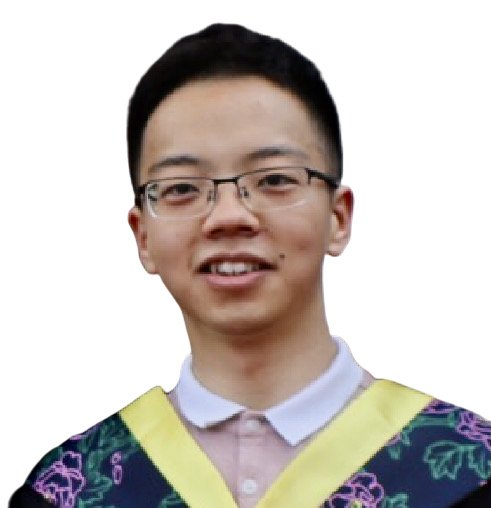
\includegraphics[width=0.95in]{me.jpeg}} & \scshape{Xueyao Zhang(张雪遥)} &  \\
    & \email{zhangxueyao19s@ict.ac.cn} & \phone{~~(+86) 152-0390-0168} \\
    % & \phone{(+86) 152-0390-0168} &  \\
    & \faWechat{ xueyao\_98} & \github[~~github.com/RMSnow]{https://github.com/RMSnow} \\
    & \faHome{\href{https://www.zhangxueyao.com}{~~zhangxueyao.com}}
    & \faGraduationCap {\href{https://scholar.google.com/citations?user=lf1udBcAAAAJ&hl=en}{~~Google Scholar}} 
  \end{tabu}
}

\section{Education}
\datedsubsection{\textbf{Institute of Computing Technology, Chinese Academy of Sciences}}{Sept. 2019 -- Jun. 2022}
{
  \small 
  % 前瞻实验室,研究方向:虚假新闻检测、事实核查,导师:\href{http://www.ict.cas.cn/sourcedb_2018_ict_cas/cn/jssrck/201011/t20101123_3028158.html}{曹娟}研究员;GPA:3.79 / 4.00.
\begin{itemize}
  \item Master candidate in Computer Application Technology (Being recommended for admission)
  \item Areas of Study: Fake News Detection
  \item Advisor: Professor Juan Cao
  \item GPA: 3.79 / 4.00
\end{itemize}
}

\datedsubsection{\textbf{School of Computer Science, Wuhan University}}{Sept. 2015 -- Jun. 2019}
{
  \small 
  % GPA:3.84 / 4.00,专业排名:4 / 246,英语六级:522.
\begin{itemize}
  \item B.Eng in Software Engineering
  \item GPA: 3.84 / 4.00, Ranking: 4 / 246 (Top 1.6\%)
\end{itemize}
}


\section{Publications}
\textbf{\large \framebox[1.2\width]{Fake News Detection}}

\datedsubsection{\textbf{1.} \quad \textit{\textbf{Mining Dual Emotion for Fake News Detection} (Long Paper; Oral)}}{}
{\small \role{\textbf{\underline{Xueyao Zhang}}, Juan Cao, Xirong Li, Qiang Sheng, Lei Zhong, Kai Shu.}{Proceedings of the 30th Web Conference \textbf{(WWW 2021)}
}
\small
\textit{TL;DR}: We leverage both publisher emotion and social emotion for fake news detection.

\datedsubsection{\textbf{2.} \quad \textit{\textbf{Integrating Pattern- and Fact-based Fake News Detection via Model Preference Learning} (Long Paper; Oral)}}{}
{\small \role{Qiang Sheng*, \textbf{\underline{Xueyao Zhang}}*, Juan Cao, Lei Zhong. (*: Equal Contribution)}{Proceedings of the 30th ACM International Conference on Information and Knowledge Management \textbf{(CIKM 2021)}}
}
\small
\textit{TL;DR}: We propose a graph-based model preference learning framework to separately handle the pattern and fact indicators in fake news detection.

\datedsubsection{\textbf{3.} \quad \textit{\textbf{Article Reranking by Memory-enhanced Key Sentence Matching for Detecting Previously Fact-checked Claims} (Long Paper; Poster)}}{}
{\small \role{Qiang Sheng, Juan Cao, \textbf{\underline{Xueyao Zhang}}, Xirong Li, Lei Zhong.}{Proceedings of the Joint Conference of the 59th Annual Meeting of the Association for Computational Linguistics \textbf{(ACL 2021)}}
\small
\textit{TL;DR:} We detect previously fact-checked claims by matching them against the key sentences in fact-checking articles.

\datedsubsection{\textbf{4.} \quad \textit{\textbf{Zoom Out and Observe: News Environment Perception for Fake News Detection}}}{}
{\small \role{Qiang Sheng, Juan Cao, \textbf{\underline{Xueyao Zhang}}, Rundong Li, Danding Wang, Yongchun Zhu.}{\textbf{(Under Review)}}
\small
\textit{TL;DR}: We leverage the external news environment where a news post is created and disseminated for detecting fake news.

\textbf{\\ \large \framebox[1.2\width]{Music Generation}}
\datedsubsection{\textbf{1.} \quad \textit{\textbf{Structure-Enhanced Pop Music Generation via Harmony-Aware Learning}}}{}
{\small \role{\textbf{\underline{Xueyao Zhang}}, Jinchao Zhang, Yao Qiu, Li Wang, Jie Zhou.}{\textbf{(Under Review)}}
}
\small
\textit{TL;DR}: We propose to learn harmony for generating form- and texture- enhanced pop music.

\section{Internship}
\datedsubsection{\textbf{腾讯 - WXG(微信事业群) - 模式识别中心}}{2021.04 -- 至今}
{\small \role{部门总监:周杰;直属领导:张金超.}{\textbf{音乐生成算法实习生}}
}
\small
\begin{itemize}
  % \item \textit{业务场景} \quad 为微信视频号中用户上传的视频自动配乐.
  \item 负责音乐生成算法的研发;提供音乐背景、乐理知识等支持,专业化地评估人工智能音乐.
  \item 举办了一次内部的音乐培训讲座:\href{https://www.zhangxueyao.com/data/wcpr-pop-music.pdf}{\underline{一首流行歌是如何创作?}}
\end{itemize}

\section{音乐能力}
\small
\begin{itemize}
  \item 掌握基础的乐理知识,熟悉常见的音乐风格.
  \item 熟悉流行音乐的键盘演奏,了解吉他演奏.
  \item 爱好流行演唱,曾获中国科学院大学校园歌手大赛季军;拥有合唱团演唱、领唱经历.
  \item 对计算音乐学、音乐生成、音乐理解等领域具有浓厚的兴趣. 
\end{itemize}

\section{编程技能}
\small
\begin{itemize}
  \item 编程语言:熟练使用Python,了解Java、C++.
  \item 深度学习框架:PyTorch、Keras.
\end{itemize}

\section{获奖情况}
\begin{itemize}
  \item 中国科学院大学校园歌手大赛季军(2020)
  \item 中国科学院大学计算机学院三好学生(2019;2020)
  \item 武汉大学优秀学士学位论文(2019)
  \item 武汉大学三好学生、优秀团员、优秀学生干部(2016;2017;2018)
  \item 本科生国家奖学金(2016)
  \item 全国高中生数学联赛一等奖(2014)
\end{itemize}

\end{document}
